\documentclass[letterpaper]{article} % DO NOT CHANGE THIS
\usepackage[submission]{aaai2027} % DO NOT CHANGE THIS
\usepackage[hyphens]{url} % DO NOT CHANGE THIS
\usepackage{graphicx} % DO NOT CHANGE THIS
\graphicspath{{images/}}
\urlstyle{rm} % DO NOT CHANGE THIS
\def\UrlFont{\rm} % DO NOT CHANGE THIS
\usepackage{natbib} % DO NOT CHANGE THIS
\usepackage{caption} % DO NOT CHANGE THIS
\frenchspacing % DO NOT CHANGE THIS

\usepackage{amsmath}
\usepackage{amssymb}
\usepackage{booktabs}

\pdfinfo{
/TemplateVersion (2027.1)
}

\setcounter{secnumdepth}{0}
% Generated from Stage 2 v2 JSON. Do not edit empirical values by hand.
\newcommand{\EffectSliceTaskCount}{2}
\newcommand{\EffectSliceReplicatesPerTask}{18}
\newcommand{\EffectSliceProviderConversations}{108}
\newcommand{\EffectSliceHiddenChecksPerRun}{64}
\newcommand{\EffectSliceAdmissions}{0}
\newcommand{\SnapMFSEBSuccesses}{0}
\newcommand{\SnapMFSEFSuccesses}{13}
\newcommand{\SnapMFSESSuccesses}{5}
\newcommand{\SnapMFSEFullBenefitSuccesses}{13}
\newcommand{\SnapMFSEFullBenefitCPLower}{0.454}
\newcommand{\SnapMFSESlicePreservationSuccesses}{3}
\newcommand{\SnapMFSESlicePreservationCPLower}{0.033}
\newcommand{\SnapMFSESliceBenefitSuccesses}{5}
\newcommand{\SnapMFSESliceBenefitCPLower}{0.092}
\newcommand{\SnapMFSEDecision}{Reject}
\newcommand{\ToolformerFilterBSuccesses}{0}
\newcommand{\ToolformerFilterFSuccesses}{18}
\newcommand{\ToolformerFilterSSuccesses}{6}
\newcommand{\ToolformerFilterFullBenefitSuccesses}{18}
\newcommand{\ToolformerFilterFullBenefitCPLower}{0.805}
\newcommand{\ToolformerFilterSlicePreservationSuccesses}{6}
\newcommand{\ToolformerFilterSlicePreservationCPLower}{0.127}
\newcommand{\ToolformerFilterSliceBenefitSuccesses}{6}
\newcommand{\ToolformerFilterSliceBenefitCPLower}{0.127}
\newcommand{\ToolformerFilterDecision}{Reject}


\title{EffectSlice: Run-Level Admission Tests for Paper-Derived Procedural Skills}
\author{Anonymous Submission}
\affiliations{}

\begin{document}

\maketitle

\begin{abstract}
Systems that compile research papers into executable skills promise faster
access to a paper's core mechanism, but evaluating one generated patch on many
deterministic tests does not establish that the skill reliably changes fresh
agent behavior.  Worse, a private scorer becomes development feedback if an
agent can observe it and revise the same patch.  We introduce
\textbf{EffectSlice}, an admission test that can accept candidates from any
reducer and decides whether to replace a complete
paper-derived procedural artifact with a source-grounded strict subset.
EffectSlice separates candidate discovery from confirmation, binds every input
by digest, scores a fixed patch once without returning private feedback, and
treats registered B/F/S replicate blocks---not hidden test cases---as the
analysis units.  We evaluate two paper-specific implementation tasks with
\EffectSliceReplicatesPerTask{} blocks per task
(\EffectSliceProviderConversations{} DeepSeek V3.2 API conversations); an
ordinary PC performs orchestration, execution, scoring, and evidence storage.
For SNAP-MFSE, B/F/S succeed in
\SnapMFSEBSuccesses/\SnapMFSEFSuccesses/\SnapMFSESSuccesses{} of
\EffectSliceReplicatesPerTask{} runs; for Toolformer filtering, the counts are
\ToolformerFilterBSuccesses/\ToolformerFilterFSuccesses/\ToolformerFilterSSuccesses.
The gate admits \EffectSliceAdmissions{} of \EffectSliceTaskCount{} selected
slices under all three exact run-level prevalence criteria.  The study replaces an invalid
single-patch, case-level confirmation interpretation and shows why compactness,
source grounding, and deterministic test coverage are proposals for reuse, not
evidence of reliable task-local substitution.
\end{abstract}

\section{Introduction}

Paper-reproduction agents increasingly turn research descriptions into code,
tests, and interactive systems \cite{starace2025paperbench,
zhao2025autoreproduce,miao2025paper2agent}.  Agent-skill systems similarly
compile heterogeneous evidence into reusable procedural artifacts
\cite{shen2026skillfoundry,pan2026anything2skill}.  These systems create a
practical opportunity: a researcher with an ordinary PC can call a vendor model
API, execute the generated code locally, and quickly test a paper's core
mechanism.  They also create a measurement problem.  When a shorter,
paper-derived skill appears sufficient, what evidence permits replacing the
complete artifact with it?

Three quantities are easily conflated.  \emph{Compactness} is a property of
the artifact.  \emph{Grounding} connects its instructions to the source paper.
\emph{Behavioral substitution} is a statement about what fresh agent runs do
under a locked task.  A compact, grounded artifact can still omit a condition
that matters.  Conversely, a complete artifact can fail because an agent does
not use it consistently.  Testing dozens of deterministic inputs on one patch
characterizes that patch; it does not create dozens of independent samples of
agent behavior.

Our initial protocol exposed a more direct failure.  A model could call a
private scorer, observe pass counts, revise the same patch, and call the scorer
again.  Those cases were then mistakenly treated as independent Bernoulli
trials.  The numerical records remain useful as development evidence, but the
confirmation claim does not survive audit.  This is the familiar adaptive
holdout problem in an agentic form: feedback from a nominal test set changes
the object being tested \cite{dwork2015reusableholdout,
nakkiran2018genericholdout}.

We propose \textbf{EffectSlice}, an admission protocol rather than another
reducer.  A complete paper-derived artifact $F$ must first improve fresh runs
over a no-artifact condition $B$.  A reducer may then propose a source-grounded
strict subset $S$.  After dependency-closure deletion audit and discovery, the
candidate, task, scorer, hidden suite, condition order, and runner are frozen.
Each B/F/S condition starts a fresh provider conversation.  The private scorer
runs at most once after a patch is fixed and never returns feedback to the
model.  Exact prevalence bounds are computed across registered B/F/S replicate
blocks; hidden cases are clustered checks defining each condition score.

We instantiate the protocol on two bounded implementation tasks derived from
SnapATAC2's matrix-free spectral embedding \cite{zhang2024snapatac2} and
Toolformer's API-call filtering rule \cite{schick2023toolformer}.  The study
uses DeepSeek V3.2 through the supplied vendor API while a commodity PC handles
all local work.  It comprises \EffectSliceProviderConversations{} provider
conversations and preserves failures rather than replacing them.  The point is
not that two tasks establish broad utility; they do not.  The point is that a
reusable artifact needs a run-level admission boundary capable of withholding
substitution when seemingly strong case-level evidence is not stable.

Our contributions are:
\begin{itemize}
    \item We formulate use of a compact paper-derived skill as three separate
    task-local hypotheses: full-artifact benefit, slice preservation, and slice
    benefit, evaluated over fresh matched B/F/S replicate blocks.
    \item We provide a leakage-resistant, auditable protocol combining
    deterministic source units, dependency-closure deletion audit, write-once
    evidence, digest binding, final-only private scoring, bounded retries, and
    exact run-level prevalence gates.
    \item We report an API-first study with two paper-specific tasks,
    \EffectSliceReplicatesPerTask{} registered blocks per task, and both
    positive and negative run outcomes.  The results quantify when complete and
    sliced artifacts change fresh agent success and explicitly replace the
    invalid case-level confirmation interpretation.
\end{itemize}

We do not claim global minimality, cross-paper effectiveness, local-model
inference, cost savings, or benefit to human users.  Those claims require
different experiments.

\section{Related Work}

\paragraph{Paper reproduction and paper-derived agents.}
PaperBench evaluates agents that recreate research code and execute experiments
from papers \cite{starace2025paperbench}.  AutoReproduce augments reproduction
with paper lineage \cite{zhao2025autoreproduce}, while Paper2Agent constructs
interactive agents around papers and associated code
\cite{miao2025paper2agent}.  These systems evaluate construction of a complete
artifact.  EffectSlice starts from a complete artifact and asks whether a
strict subset can be admitted as a task-local substitute.

\paragraph{Agent skills and context compilation.}
SkillFoundry and Anything2Skill compile reusable skills from heterogeneous
resources \cite{shen2026skillfoundry,pan2026anything2skill}.  Graph-of-Skills
retrieves dependency-aware bundles \cite{liu2026graphskills}; SkillRAE compiles
retrieved evidence into compact grounded execution context
\cite{meng2026skillrae}; and ClawTrace attributes costs to skill-distillation
traces and distinguishes rule types \cite{yuan2026clawtrace}.  A recent
framework measures the marginal utility of agent skills at scale
\cite{shaposhnikov2026agenticskills}.  These methods can generate, retrieve, or
score candidates.  EffectSlice is a downstream decision layer: no reducer
bypasses the same full-benefit and preservation tests.

\paragraph{Reduction and equivalence.}
Delta debugging and C-Reduce find smaller inputs that preserve an observed
failure \cite{zeller2002simplifying,regehr2012creduce}; cause reduction extends
this idea beyond crashes \cite{groce2016cause}.  Prompt-compression systems
optimize context size while measuring retained information
\cite{jiang2023llmlingua,pan2024llmlingua2}.  EffectSlice shares the
counterfactual reduction motif but conditions it on a beneficial complete
artifact and evaluates the selected subset on fresh agent runs.  Its gate uses
an explicit equivalence tolerance \cite{wellek2002equivalence} and exact
binomial bounds \cite{clopper1934binomial}.

\paragraph{Adaptive evaluation.}
Repeatedly exposing holdout information can overfit an adaptively chosen
hypothesis even when the nominal test data are separate from training data
\cite{dwork2015reusableholdout}.  Limited-exposure holdouts therefore reveal
only the decision needed to validate a fixed hypothesis
\cite{nakkiran2018genericholdout}.  EffectSlice applies this principle to
tool-using agents: discovery may be interactive, but confirmation fixes the
patch before one private score and terminates without another model turn.

\section{Problem Formulation}

Let $B$ denote a same-scaffold condition with no paper-derived procedures,
$F=\{a_1,\ldots,a_K\}$ the complete source-grounded artifact, and
$S\subset F$ a nonempty strict subset proposed after discovery.  We use
\emph{skill} operationally to mean a finite, ordered collection of
source-grounded procedural instructions injected into one fixed condition
context slot; it is not model memory or a model-independent statement of a
paper's unique core.  Each condition
run starts a fresh provider conversation under a locked task, workspace, action
budget, and scorer.  A private suite of
\EffectSliceHiddenChecksPerRun{} deterministic cases produces a task score
$q_{A,r}\in[0,1]$ for condition $A\in\{B,F,S\}$ in registered block $r$.
The cases define one clustered score; they are not independent samples of the
agent.

Let $h_{A,r}$ indicate that all task contracts and guardrails pass.  A condition
run succeeds when
\begin{equation}
z_{A,r}=\mathbb{1}\left[h_{A,r}=1 \;\land\; q_{A,r}\geq 0.95\right].
\end{equation}
Missing patches, exhausted provider retries, missing scores, and contract
failures yield $z_{A,r}=0$ and remain in the registered denominator.

For each block, EffectSlice evaluates three indicators:
\begin{align}
g^{F}_{r} &=
  \mathbb{1}[z_{F,r}=1 \land z_{B,r}=0],\\
g^{P}_{r} &=
  \mathbb{1}[z_{S,r}=z_{F,r}]
  \mathbb{1}[|q_{S,r}-q_{F,r}|\leq 0.05],\\
g^{S}_{r} &=
  \mathbb{1}[z_{S,r}=1 \land z_{B,r}=0].
\end{align}
They represent full-artifact benefit, slice preservation, and slice benefit.
If a required score is missing, every indicator that uses it is set to zero.
The decision is task-local: it concerns one paper-derived artifact, task,
provider configuration, scorer, and registered run population.

\section{EffectSlice}

\subsection{Gate 1: Full-Artifact Benefit}

No subset is considered until the complete artifact has a measurable advantage
over no artifact.  On the final registered schedule, this is the
$g^F$ indicator above, rather than a count of cases passed by one patch.
Separating this gate prevents a reducer from preserving an artifact that its
complete form does not reliably make useful.

\subsection{Gate 2: Source-Grounded Candidate Registry}

Each procedural unit records an identifier, a paper-derived text span, an
executable role, dependency edges, and an artifact digest.  A candidate must be
a strict nonempty subset, contain only registered units, satisfy dependency
closure, and compile into the same task interface as $F$.  The current
instantiation uses five units per paper and a deliberately simple ordered-prefix
reducer.  In both tasks the five singleton strongly connected components form a
dependency chain, so dependency-closed candidates are prefixes.  SNAP-MFSE
selects a three-unit prefix; Toolformer filtering selects a
one-unit prefix.  The reducer is not the contribution: it creates concrete
candidates on which to test the admission protocol.

\subsection{Gate 3: Discovery and Closure-Deletion Audit}

Discovery evaluates candidates in frozen increasing-size order.  Once a
candidate agrees with $F$ on the discovery block and passes the task contract,
it is locked.  For every retained unit, the audit removes that unit and
cascades removal of retained units that transitively require it.  Every
resulting registered dependency-closed neighbor must fail the discovery
criterion.  This establishes local indispensability under the registered
closure operator; it does not establish global minimality under arbitrary
rewrites.

Discovery scores are development evidence.  They can choose a candidate but
cannot confirm it.  This distinction is especially important for agent runs:
an apparently perfect candidate on one generated patch can be unreliable in a
fresh conversation.

\subsection{Gate 4: Final-Only Run-Level Confirmation}

Confirmation uses \EffectSliceReplicatesPerTask{} registered B/F/S blocks per
task.  The six condition permutations each occur three times in a fixed
shuffled schedule.  Before the first provider call, a family manifest binds the
task prompt, workspace tree, complete artifact, source map, selected slice,
slice registry, discovery summary, hidden-case registry, scorer, runner,
scheduler, transport, thresholds, block identifiers, and condition orders by
SHA-256.

The model may search, open, and edit the public workspace.  A \texttt{test}
action is unavailable in confirmation and never invokes the private scorer.
\texttt{submit} fixes the patch, invokes the scorer once, and terminates.  If
the action budget expires with a nonempty patch, that final patch is scored
once; an empty patch fails without a scorer call.  The result records the score
count, whether private feedback was exposed, provider response identity, and a
complete transcript.  Output directories are write-once.

For indicator $g\in\{g^F,g^P,g^S\}$, let $k_g$ be its successes among
$n=\EffectSliceReplicatesPerTask{}$ registered blocks.  We compute the
one-sided Clopper--Pearson lower bound
\begin{equation}
L_g=\mathrm{Beta}^{-1}(0.02;k_g,n-k_g+1).
\end{equation}
The slice is admitted only if every $L_g>0.8$, every hard contract passes, and
the integrity audit succeeds.  With the registered $n$, 18/18 gives
$L=0.8047$; one failed block is sufficient to withhold admission.  Thresholds
are not changed after observing outcomes.

\section{Experimental Setup}

\subsection{Paper-Specific Tasks}

\paragraph{SNAP-MFSE.}
The task implements the matrix-free spectral embedding core described by
SnapATAC2 \cite{zhang2024snapatac2}: inverse-document-frequency scaling, row
normalization, self-similarity removal and degree construction, linear-operator
exposure, and leading spectral coordinates.  The hidden scorer checks numerical
behavior, the function contract, and a matrix-free guard over varied clustered
count matrices.

\paragraph{Toolformer filtering.}
The task implements Toolformer's rule for retaining proposed API calls
\cite{schick2023toolformer}: normalized future-token weights, weighted losses,
the stronger counterfactual baseline, thresholding, and ordered application to
all proposals.  The v2 suite varies candidate count, horizon, thresholds,
counterfactual losses, and expected keep patterns.  An earlier development
contract omitted edge-case conventions; that lineage is preserved but excluded
from confirmation.

For both tasks, B, F, and S share the task prompt, workspace, action interface,
action budget, hidden suite, and deterministic scorer.  Only the injected
paper-derived artifact changes.  Each condition has at most 16 model actions.

\subsection{API-First Commodity-Device Execution}

The primary inference service is the user-supplied DeepSeek endpoint.  We use
the provider/user label DeepSeek V3.2 and disclose the exact request alias
\texttt{deepseek-v4-flash}; the alias-to-deployment mapping is not independently
attested.  Requests use OpenAI-compatible chat completions, temperature zero,
and task-specific output limits.  Response model fields, response IDs, creation
times, token counts, and retry lineages are stored.

A local ordinary PC performs orchestration, bounded code execution,
deterministic scoring, integrity checks, and artifact persistence.  Model
inference remains at the vendor endpoint; no local GPU, quantized model, or
large local accelerator is part of the experiment.  This setting reflects the
common API-first meaning of commodity-device use, not local inference.
The recorded host has a 16-core Ryzen 9 7945HX, 31.7~GiB RAM, and an
8~GiB RTX 4060 Laptop GPU; the GPU is incidental and is not used for model
inference.

Connection errors, timeouts, HTTP 429, and transient 5xx responses are retried
up to five times within the same model turn.  Exhausted failures are not
replaced.  The provider exposes no supported random seed, so we claim fresh
sessions and balanced order, not seeded determinism.

\subsection{Units and Evidence Boundaries}

The experiment contains \EffectSliceProviderConversations{} provider
conversations arranged into
$\EffectSliceTaskCount\times\EffectSliceReplicatesPerTask$ matched B/F/S
blocks.  A conversation is the condition-run source; a matched block is the
Bernoulli analysis unit for each paired indicator.  The
\EffectSliceHiddenChecksPerRun{} hidden cases inside a condition are clustered
checks.  Old interactive confirmation results are labeled
\texttt{contaminated\_development} and excluded from every v2 count, bound, and
decision.

\section{Results}

\begin{figure*}[t]
\centering
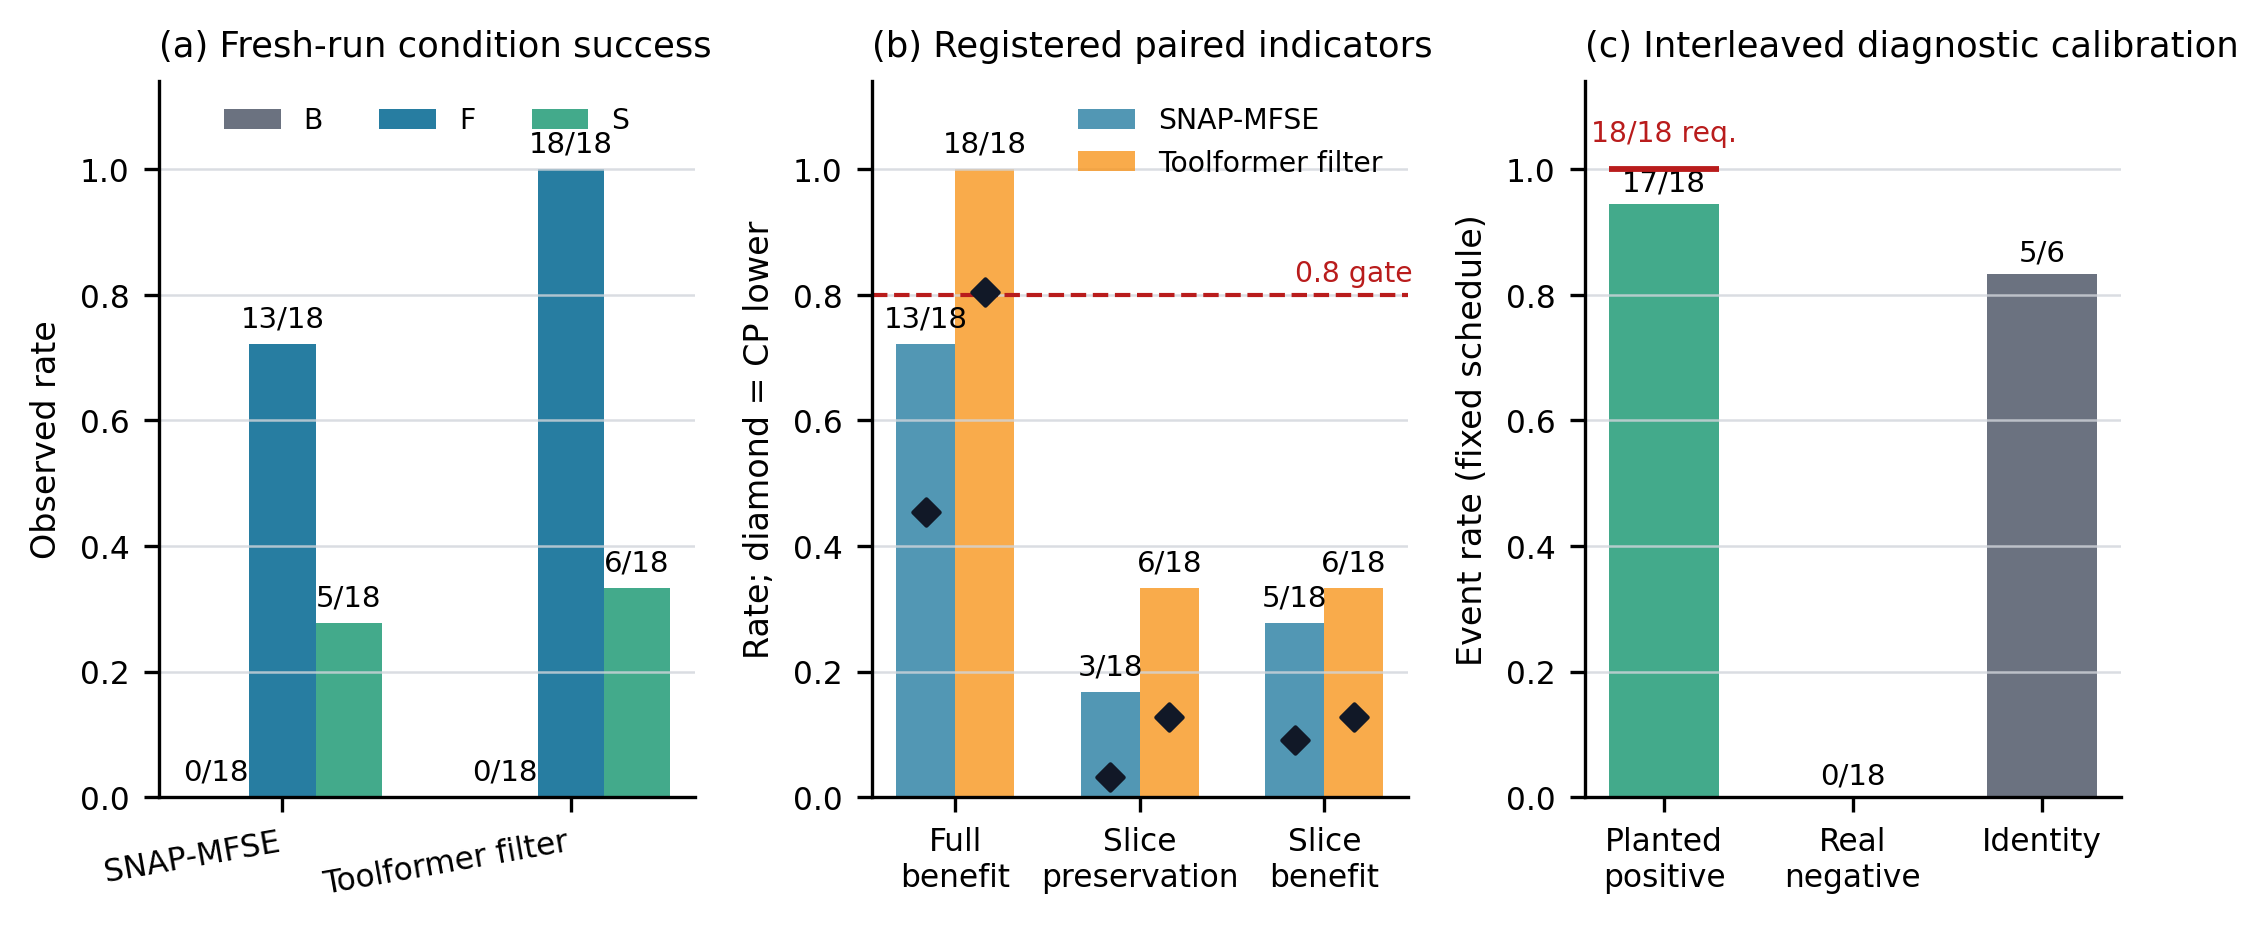
\includegraphics[width=\textwidth]{effectslice_run_level_evidence.png}
\caption{Run-level evidence derived from v2 JSON summaries.  (a) Successful
condition runs under no artifact (B), the complete paper-derived artifact (F),
and the selected slice (S).  (b) Success rates of the three registered matched
indicators; diamonds are one-sided 98\% Clopper--Pearson lower bounds, and the
dashed line is the 0.8 admission threshold.  Each bar uses 18 matched blocks per
task.  Hidden cases define within-run scores and are not independent bars.}
\label{fig:runlevel}
\end{figure*}

\begin{table*}[t]
\centering
\caption{Confirmation-v2 outcomes.  Counts are successful independent
condition runs or matched-block indicators out of
\EffectSliceReplicatesPerTask; parentheses give one-sided CP lower bounds.
All values are generated from the final v2 summaries.}
\label{tab:results}
\begin{tabular}{lccccc}
\toprule
Task & B/F/S successes & Full benefit & Slice preservation & Slice benefit & Gate \\
\midrule
SNAP-MFSE &
\SnapMFSEBSuccesses/\SnapMFSEFSuccesses/\SnapMFSESSuccesses &
\SnapMFSEFullBenefitSuccesses\ (\SnapMFSEFullBenefitCPLower) &
\SnapMFSESlicePreservationSuccesses\ (\SnapMFSESlicePreservationCPLower) &
\SnapMFSESliceBenefitSuccesses\ (\SnapMFSESliceBenefitCPLower) &
\SnapMFSEDecision \\
Toolformer filter &
\ToolformerFilterBSuccesses/\ToolformerFilterFSuccesses/\ToolformerFilterSSuccesses &
\ToolformerFilterFullBenefitSuccesses\ (\ToolformerFilterFullBenefitCPLower) &
\ToolformerFilterSlicePreservationSuccesses\ (\ToolformerFilterSlicePreservationCPLower) &
\ToolformerFilterSliceBenefitSuccesses\ (\ToolformerFilterSliceBenefitCPLower) &
\ToolformerFilterDecision \\
\bottomrule
\end{tabular}
\end{table*}

\subsection{Artifacts Change Fresh-Run Success Non-Uniformly}

Figure~\ref{fig:runlevel}(a) reports condition success before any paired
interpretation.  For SNAP-MFSE, B succeeds in \SnapMFSEBSuccesses{} runs, F in
\SnapMFSEFSuccesses, and S in \SnapMFSESSuccesses{} out of
\EffectSliceReplicatesPerTask.  For Toolformer filtering, the corresponding
counts are \ToolformerFilterBSuccesses, \ToolformerFilterFSuccesses, and
\ToolformerFilterSSuccesses.  These are session-level outcomes: each patch is
generated afresh, then scored on the same private case registry.

The spread matters.  A full artifact may encode the correct procedure yet fail
to influence every bounded conversation.  A slice may occasionally succeed
when its matched full condition does not, without thereby establishing
preservation.  Condition success rates alone therefore cannot answer the
substitution question.

\subsection{The Three Gates Separate Benefit from Preservation}

The full-benefit indicator holds in
\SnapMFSEFullBenefitSuccesses/\EffectSliceReplicatesPerTask{} SNAP blocks and
\ToolformerFilterFullBenefitSuccesses/\EffectSliceReplicatesPerTask{}
Toolformer blocks; their lower bounds are
\SnapMFSEFullBenefitCPLower{} and
\ToolformerFilterFullBenefitCPLower.  Slice preservation holds in
\SnapMFSESlicePreservationSuccesses{} and
\ToolformerFilterSlicePreservationSuccesses{} blocks, with lower bounds
\SnapMFSESlicePreservationCPLower{} and
\ToolformerFilterSlicePreservationCPLower.  Slice benefit holds in
\SnapMFSESliceBenefitSuccesses{} and
\ToolformerFilterSliceBenefitSuccesses{} blocks, with lower bounds
\SnapMFSESliceBenefitCPLower{} and
\ToolformerFilterSliceBenefitCPLower.

The final decisions are \SnapMFSEDecision{} for SNAP-MFSE and
\ToolformerFilterDecision{} for Toolformer filtering.  In total,
\EffectSliceAdmissions/\EffectSliceTaskCount{} selected slices are admitted.
An admission is a local substitution record under this task, provider, prompt,
scorer, and run schedule; a rejection means the available evidence is
insufficient under the frozen gate, not that the source paper's mechanism is
incorrect.

\subsection{Why the Earlier Confirmation Interpretation Is Excluded}

The historical implementation let the model invoke the confirmation scorer,
observe private pass information, and continue editing.  It then treated the
hidden cases for one final patch as independent trials.  Confirmation v2 changes
both the information flow and the analysis unit: scoring is terminal and the
denominator is a set of fresh matched blocks.  We preserve the old bundles for
audit but do not combine their values with Table~\ref{tab:results}.  The
difference is methodological, not a post-hoc deletion of unfavorable runs.

\section{Discussion}

\paragraph{A paper-derived core is a hypothesis about agent behavior.}
Source grounding answers where an instruction came from.  Dependency closure
answers whether registered prerequisites were retained.  Neither guarantees
that a stochastic agent will use the artifact.  EffectSlice therefore treats a
compact core as a candidate whose substitution claim must survive fresh runs.

\paragraph{Rejection is a useful output.}
A workflow aimed at rapid paper reproduction should be able to say that the
complete artifact is not reliably beneficial, or that a selected subset does
not preserve its behavior.  Otherwise, the workflow converts every successful
single patch into a reusable skill and hides instability.  The strict 18/18
prevalence gate intentionally favors false abstention over unsupported
replacement.

\paragraph{Why the ordinary-device boundary is API-first.}
The research question is artifact admission, not local model serving.  Requiring
a local quantized model would add capability and quantization confounds
unrelated to the gate.  A commodity PC plus a trusted vendor API is the relevant
operational baseline for ordinary researchers today.  Vendor dependence remains
a threat, but local model deployment is not a prerequisite for this protocol.

\paragraph{Relation to fast reproduction.}
EffectSlice can sit after a paper-to-code or paper-to-agent system: extract the
paper-specific procedure, propose a smaller dependency-closed core, run B/F/S
blocks through the provider API, and either expose the core with its evidence
boundary or retain the complete artifact.  Our experiment tests the technical
admission decision.  It does not test whether nonexpert people finish their own
projects faster.

\section{Limitations and Threats to Validity}

\paragraph{External validity.}
The study contains two source papers, two bounded code-generation tasks, one
provider service, and one prompt/scaffold family.  The tasks isolate
paper-specific mechanisms rather than reproducing full biological analyses or
language-model training.  No cross-paper admission rate follows.
All conversations for a task use the same hidden-case registry, so the exact
bounds concern provider-session variability conditional on that registry; they
do not estimate performance over a population of hidden-case generators.

\paragraph{Operational independence.}
Each condition starts a fresh API conversation, but the provider does not expose
a seed or guarantee independent backend sampling.  Shared infrastructure,
caching, model updates, or undisclosed routing can induce dependence.  Balanced
condition order reduces one systematic effect but cannot certify statistical
independence.

\paragraph{Power and gate strictness.}
At $n=18$ and $\alpha=0.02$, the 0.8 lower-bound gate requires 18/18 indicator
successes.  This makes an admission easy to interpret but has low power and can
reject useful artifacts.  Larger registered schedules or hierarchical models
would support graded reliability estimates; changing the threshold after
seeing these results would not.

\paragraph{Task-contract sensitivity.}
The Toolformer development history shows that edge-case conventions can
dominate scores.  Source grounding does not eliminate ambiguity when paper
prose is translated into an executable contract.  Independent contract review
and more task families are needed.

\paragraph{Reducer and baseline coverage.}
The ordered-prefix reducer exercises the gate but does not compare search
quality against Graph-of-Skills, SkillRAE, ClawTrace, or other candidate
generators.  EffectSlice is compatible with those reducers, but superiority is
untested.

\paragraph{Efficiency and user benefit.}
We do not claim fewer model actions, lower token cost, faster wall-clock
completion, or improved human understanding.  No human participants were
studied.  Those outcomes require matched cost measurements and a user study.

\section{Broader Impact}

Admission tests can reduce overconfident reuse of compact paper-derived
instructions by making abstention and negative evidence first-class outputs.
They can also create false assurance if a local decision is generalized beyond
its paper, task, provider, scorer, or time window.  Every result should expose
those boundaries and retain raw evidence.  Generated code remains a
supply-chain risk; bounded workspaces and private scoring reduce, but do not
remove, that risk.

\section{Conclusion}

EffectSlice reframes a compact paper-derived skill as a task-local substitution
hypothesis.  Complete-artifact benefit, source binding, dependency-closure
audit, final-only private scoring, and run-level exact bounds determine whether
the candidate may replace the full artifact.  Across
\EffectSliceProviderConversations{} DeepSeek API conversations, the two tasks
show that correct-looking, case-tested procedures need not influence fresh
agent runs uniformly.  A credible fast-reproduction workflow therefore needs
more than extraction and deterministic tests: it needs an admission rule that
can preserve negative evidence and say no.

\bibliography{effectslice_refs}

\end{document}
